\documentclass[10pt]{beamer}
\usepackage[utf8]{inputenc}
%\usepackage[dvipsnames]{xcolor}
\usepackage{charter}
\usepackage{amsmath}
\usepackage{amsfonts}
\usepackage{mathtools}
\usepackage{amssymb}
\usepackage{hyperref}
\usepackage[ruled,vlined]{algorithm2e}
\usepackage{commath}

\newcommand\pro{\item[\textbf{+}]}
\newcommand\con{\item[\textbf{--\kern 1.2pt}]}

% justify text in bibliography
\usepackage{ragged2e}  % for \justifying
\usepackage{etoolbox}
\apptocmd{\thebibliography}{\justifying}{}{}
\usepackage{natbib} 
\bibliographystyle{plainnat}
% links in blue
\definecolor{links}{HTML}{2A1B81}
\hypersetup{colorlinks=true,citecolor=blue,linkcolor=,urlcolor=links}
\addtobeamertemplate{navigation symbols}{}{%
    \usebeamerfont{footline}%
    \usebeamercolor[fg]{footline}%
    \hspace{1em}%
    \insertframenumber
}
\setbeamercolor{footline}{fg=black}

\title{Stochastic variance reduced gradient methods for training Deep Neural Networks}
\author{Alexander Apostolov}
\institute {École Polytechnique Fédérale de Lausanne}
\date{February $1^{st}$ 2021}

\begin{document}

\begin{frame}{ }
    \maketitle
    \begin{center}
        Project advised by:\\
        Dr. Tatjana Chavdarova, Supervisor \\
        Prof. Dr. Martin Jaggi, Advising Professor
    \end{center}
\end{frame}

\begin{frame}{}
    Empirical study of  \textbf{stochastic variance reduced gradient methods}\footnote{Herein referred as \textit{Variance Reduced},  for short. } on  training \textbf{deep neural networks} (DNNs).
\end{frame}

\begin{frame}{ }
    \begin{center}
        \Huge Background
    \end{center}
\end{frame}

\begin{frame}
\frametitle{Why variance reduction methods?}
\begin{itemize}
    \item In machine learning, the following optimization is often encountered.\
    Let $w$ denote the model parameters, and let $f_1, f_2, \dots, f_n$ be a sequence of vector functions $\mathbb{R}^d \mapsto \mathbb{R}$ where each $f_i(\cdot)$ is the loss on a single training data point.
    The goal is to find a solution to the following \textbf{finite-sum} problem:
    $$\min_w F(w),~~F(w)=\frac{1}{n}\sum_{i=1}^n f_i(w)\,.$$
    \item \textbf{Gradient Descent (GD)} is an iterative method, where at each step $ t=1, \dots, T$:
    $$w^{(t)} = w^{(t-1)} - \eta_t \nabla F(w^{(t-1)}) \,,$$\
    where $\eta_t$ is the learning rate at iteration $t$.
    \item Each iteration requires computation of the whole gradient, this is why \textbf{Stochastic Gradient Descent (SGD)}--which decreases  the computational cost by $\frac{1}{n}$ per iteration, has been widely adopted:
    $$w^{(t)} = w^{(t-1)} -\eta_t \nabla f_{i_t}(w^{(t-1)})\,.$$
\end{itemize}
\end{frame}

\begin{frame}{Why variance reduction methods?}
    Taking a sub-sample of the full dataset in SGD increases the variance of the gradient estimates, which in turn slows down convergence (in terms of parameter updates). 
    
    \vspace{5mm}
    This creates a trade off between fast per iteration computation and fast convergence.
    
    \vspace{5mm}
    \textbf{Variance reduced methods} allow keeping fast convergence at fast per iteration speed. We will analyze two methods:
    \begin{itemize}
        \item \textbf{Stochastic Variance Reduced Gradient (SVRG)}~\citep{johnson2013svrg}
        \item \textbf{STOchastic Recursive Mometum (STORM)}~\citep{Cutkosky2019storm}
    \end{itemize}
    
\end{frame}

\begin{frame}{SVRG}
    Each iteration of SVRG is given by:
    $$w^{(t)} = w^{(t-1)} -\eta(\nabla f_{i_t}(w^{(t-1)}) - \nabla f_{i_t}(\Tilde{w}) + \Tilde{\mu})$$
    where $\Tilde{w}$ is snapshot of $w$ taken when $\Tilde{\mu}$ is computed every $m$ iterations, and:
    $$\Tilde{\mu} = \nabla F(\Tilde{w}) = \frac{1}{n}\sum_{i=1}^n \nabla f_i(\Tilde{w})$$
\end{frame}


\begin{frame}{SVRG}
    \begin{algorithm}[H]
    \DontPrintSemicolon
    \SetAlgoNoLine
    
    \KwIn{learning rate $\eta$ and update frequency $m$}
    \textbf{Initialize} $\Tilde{w}_0$\;
    \For{$epoch \leftarrow 1, 2, \dots$}{
      $\Tilde{w} \gets \tilde{w}_{epoch-1}$\;
      $\Tilde{\mu} \gets \frac{1}{n}\sum_{i=1}^n \nabla f_i(\Tilde{w})$\;
      $w^{(0)} \gets \tilde{w}$\;
      \For{$t \leftarrow 1,2\dots, T$}{
        Randomly pick $i_t \in \{1, \dots, n\}$  
        
        $w^{(t)} \gets w^{(t-1)} -\eta(\nabla f_{i_t}(w^{(t-1)}) - \nabla f_{i_t}(\Tilde{w}) + \Tilde{\mu})$
      }
      \textbf{Save snapshot} $\tilde{w}_{epoch} \gets w_T$\;
    }
    \caption{{\textsc{SVRG Procedure}}}
    \label{algo:svrg}
\end{algorithm}
\end{frame}

\begin{frame}{SVRG}
    Notice that: 
    \begin{itemize}
        \item $\nabla f_{i_t}(w^{(t-1)}) - \nabla f_{i_t}(\Tilde{w}) + \Tilde{\mu}$ is an unbiased estimate of $\nabla F(w)$:
    $$\mathbb{E}[w^{(t)} | w^{(t-1)}] = w^{(t-1)}-\eta_t \nabla F(w^{(t-1)})$$
        \item Variance is reduced. When $\Tilde{w}$ and $w^{(t)}$ both converge to $w_{\ast}$, then $\Tilde{\mu} \rightarrow 0$. If $\nabla f_i(\Tilde{w}) \rightarrow \nabla f_i(w_{\ast})$, then:
        $$\nabla f_i(w^{(t-1)}) - \nabla f_i(\Tilde{w}) + \Tilde{\mu} \rightarrow \nabla f_i(w^{(t-1)}) - \nabla f_i(w_{\ast}) \rightarrow 0$$
    \end{itemize}
\end{frame}

\begin{frame}{STORM}
    Each iteration of STORM is given by:
    $$d^{(t)} = (1-a)d^{(t-1)} + a\nabla f_{i_t}(w^{(t)}) + (1-a)(\nabla f_{i_t}(w^{(t)}) +  \nabla f_{i_t}(w^{(t-1)}))$$
    $$w^{(t+1)} = w^{(t)} - \eta_t d_t$$
    Notice that:
    \begin{itemize}
        \item When $w^{(t)} \approx w^{(t-1)}$, then the last term of the first equality tends to 0. 
    \end{itemize}
\end{frame}

\begin{frame}{STORM}
    \begin{algorithm}[H]
    \DontPrintSemicolon
    \SetAlgoNoLine

    \KwIn{Hyperparameters $k, w, c$}
    \textbf{Initialize} $w_1$\;
    $G_1 \gets \mathopen| {\nabla f_{i_1}(w_1)}\mathclose|$\;
    $d_1 \gets \nabla f_{i_1}(w_1)$\;
    \For{$t \leftarrow 1, 2, \dots$}{
        $\eta_t  \gets \frac{k}{(w_t+\sum_{i=1}^tG_i^2)^{1/3}}$\;
        $w_{t+1} \gets w_t - \eta_t d_t$\;
        $a_{t+1} \gets c\eta_t^2$\;
        $G_{t+1} \gets \mathopen|\nabla f_{i_{t+1}}(w_{t+1})\mathclose|$\;
        $d_{t+1} \gets \nabla f_{i_{t+1}}(w_{t+1}) + (1-a_{t+1})(d_t - \nabla f_{i_{t+1}}(w_t))$\;
    }
    \caption{{\textsc{STORM Procedure}}}
    \label{algo:storm}
\end{algorithm}
\end{frame}


\begin{frame}{SVRG vs STORM}
    \begin{itemize}
        \item SVRG compared to STORM:
            \begin{itemize}
                \pro Difficult to get insight on hyperparameters $k,w \text{ and } c$ in STORM.
                \pro More hyperparameters to tune for STORM.
                \con SVRG needs a full gradient computation every m steps (every 5 epochs in non-convex problems).
            \end{itemize}
        \item Both algorithms need two gradient computations per iteration.
        \item Both algorithms do not have official PyTorch implementations.
    \end{itemize}
\end{frame}

\begin{frame}{Batch-normalization layers~\citep{ioffe2015batch}}
    \begin{itemize}
        \item Layer used to normalize the input of layers of the network with the following formula:
        \begin{equation}\label{eq:BN}\nonumber
            y = \frac{x-\mathbb{E}[x]}{\sqrt{\mathbb{V}ar[x]+\epsilon}}\,,
        \end{equation}
        \item No direct access to $\mathbb{E}[x]$ and $\mathbb{V}ar[x]$ as $x's$ are only seen throughout the training,
        \item Using running estimates for these two values by using average computations with momentum. 
        \item Breaks assumptions for unbiased estimates in variance reduced methods.
    \end{itemize}
\end{frame}

\begin{frame}{MetaInit}
    Method for weights initialization introduced in 2019~\citep{NEURIPS2019_876e8108}.
    \begin{itemize}
        \item Deep Neural networks can be difficult to train, the performance depends heavily on how weights are initialized.
        \item Hypothesis of MetaInit: start training in regions that look locally linear with minimal second order effects.
        \item MetaInit uses measures the above with a quantity called gradient quotient.
        \item The algorithm minimizes this quantity using GD to select the norms of initial weights.
    \end{itemize}
    \begin{figure}
        \centering
        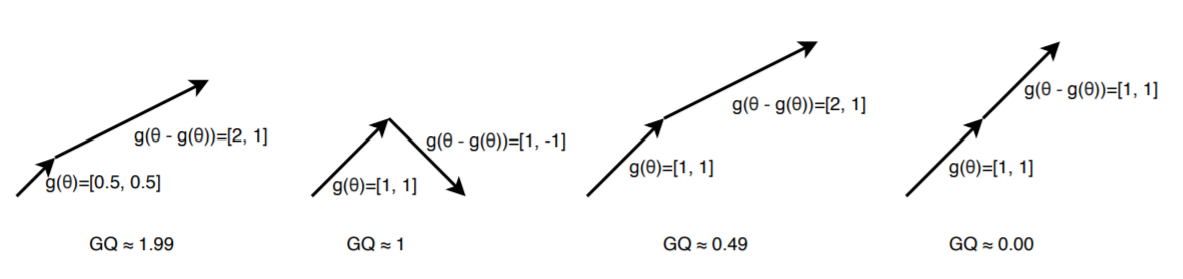
\includegraphics[width=.8\textwidth]{report/figures/MetaInit.png}
        \caption{Gradient quotient for different scenarios of initial gradient $g(\theta)$ and gradient after one update $g(\theta - g(\theta))$.}
        \label{fig:GQexample}
    \end{figure}
\end{frame}

\begin{frame}{ }
    \begin{center}
        \Huge Project motivation \& goals
    \end{center}
\end{frame}

\begin{frame}{Goal of this semester project}
    Empirical study of  \textbf{stochastic variance reduced gradient methods}\footnote{Herein referred as \textit{Variance Reduced},  for short. } on  training \textbf{deep neural networks} (DNNs).
    \newline
    \begin{itemize}
        \item Comparison between different variance reduced and stochastic methods on different architectures:
        \begin{itemize}
            \item Shallow neural network (LeNet),
            \item Deep neural network (ResNet18),
            \item Deeper neural network (ResNet101).
        \end{itemize}
        \item Goal: understand better \& potentially improve the performance of variance reduction methods for training DNNs. 
    \end{itemize}
\end{frame}



\begin{frame}{Variance reduced methods on deep neural networks}
    We want to test if variance reduced methods are still performing better on deep neural networks.
    \newline
    The paper "On the Ineffectiveness of Variance Reduced
    Optimization for Deep Learning"~\citep{Defazio2019} suggests that this is not the case, but:
    \begin{itemize}
        \item They give \textbf{no theoretical insights} why variance reduced methods perform poorly.
        \item They \textbf{use Batch-Norm Layers} in their setup. Batch-Norm layers break the assumption that the updates in SVRG are unbiased in expectation.
    \end{itemize}
\end{frame}

\begin{frame}{Hypothesis we want to test}
    \begin{itemize}
        \item Is the use of batch-normalization layers related to the failure of the stochastic variance reduced gradient (SVRG) method on deeper architectures?
        \item Can initialization methods help give better results to variance reduced methods in a setting without batch-normalization layers, by selecting better initial weights for training?
    \end{itemize}
    
\end{frame}

\begin{frame}{ }
    \begin{center}
        \Huge Experiments \& Results
    \end{center}
\end{frame}
\begin{frame}{Baseline comparison on shallow NN}
    We first performed a baseline comparison on MNIST on LeNet for the following algorithms:
    \begin{itemize}
        \item Adam~\citep{kingma2014adam},
        \item SGD
        \item AdaGrad~\citep{john2011adagrad}, 
        \item SVRG
        \item STORM
    \end{itemize}
    
    Hyperparameters selected by doing a 4-fold cross-validation.
\end{frame}

\begin{frame}{CV results example}
    \begin{figure}
        \centering
        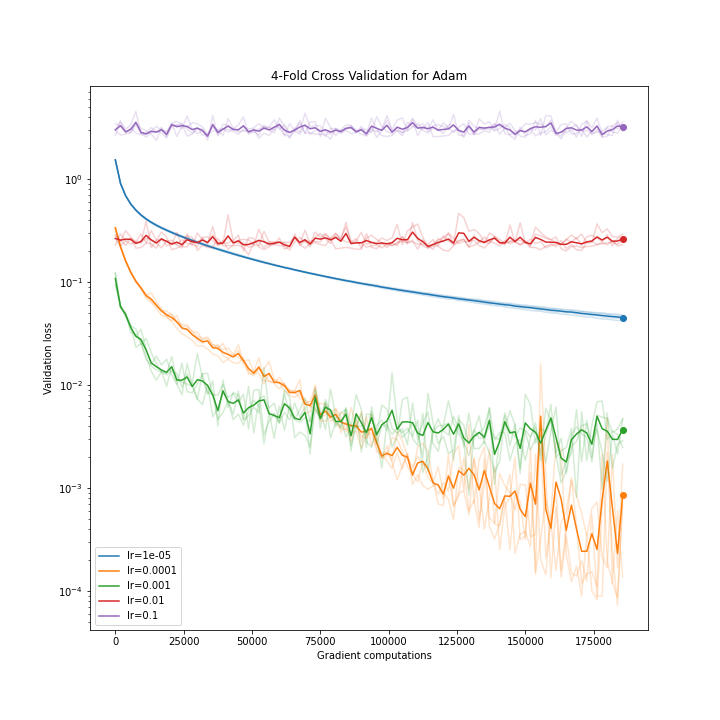
\includegraphics[width=.65\textwidth]{report/midterm presentation/images/adamCV.png}
        \caption{Cross validation of Adam on LeNet for MNIST}
        \label{fig:AdamCVLeNet}
    \end{figure}
    
\end{frame}

\begin{frame}{Results on LeNet}
    \begin{figure}
        \centering
        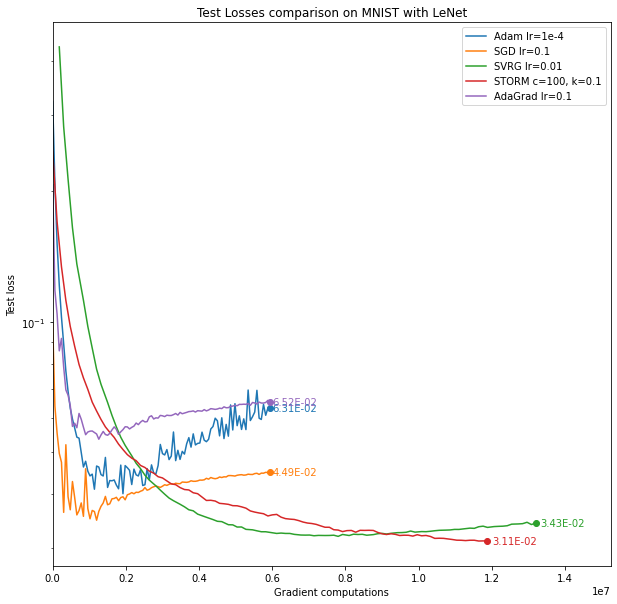
\includegraphics[width=.6\textwidth]{report/figures/MNISTresultsOnlyTest.png}
        \caption{Test losses on LeNet for MNIST}
    \end{figure}
\end{frame}

\begin{frame}{Setup for experiments on deep NN}
    \begin{itemize}
        \item ResNet18 for CIFAR10,
        \item ResNet101 for CIFAR100,
        \item Both tested with and without batch-normalization layers,
        \item Hyperparameters selected with validation set.
    \end{itemize}
\end{frame}



\begin{frame}{Results ResNet18}
     \begin{figure}
         \centering
         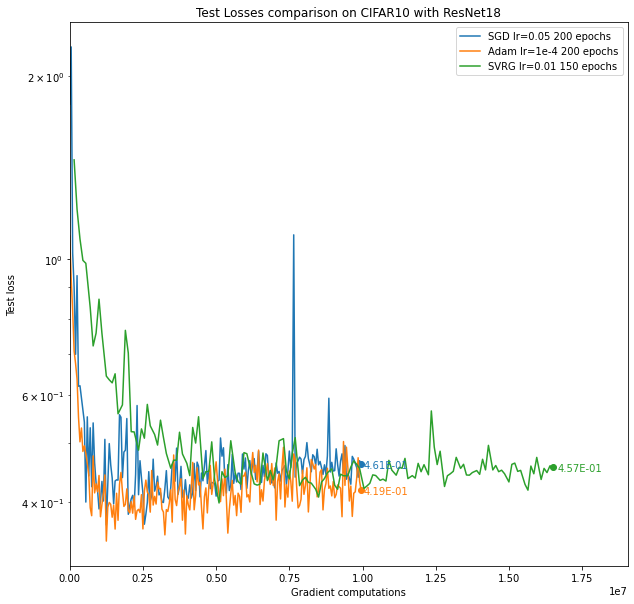
\includegraphics[scale=0.35]{report/figures/ResNet18Results.png}
         \label{fig:resnet18results}
     \end{figure}
\end{frame}

\begin{frame}{Results ResNet18 without BN}
     \begin{figure}
         \centering
         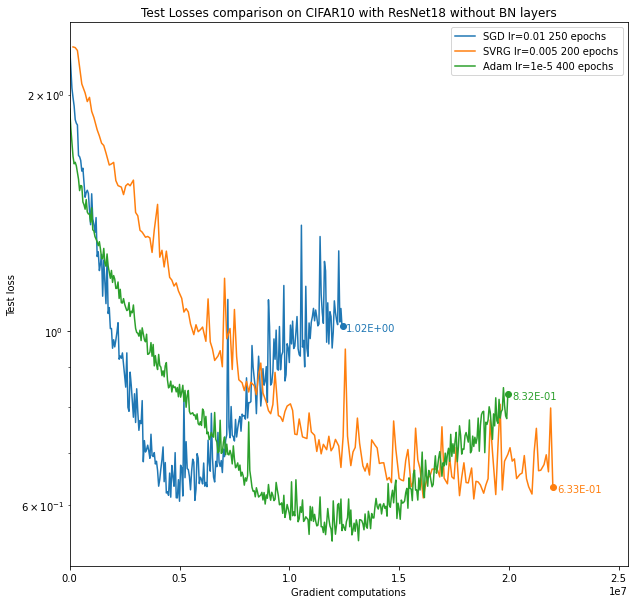
\includegraphics[scale=0.35]{report/figures/ResNet18noBNResults.png}
         \label{fig:resnet18noBNresults}
     \end{figure}
\end{frame}

\begin{frame}{Results ResNet101}
     \begin{figure}
         \centering
         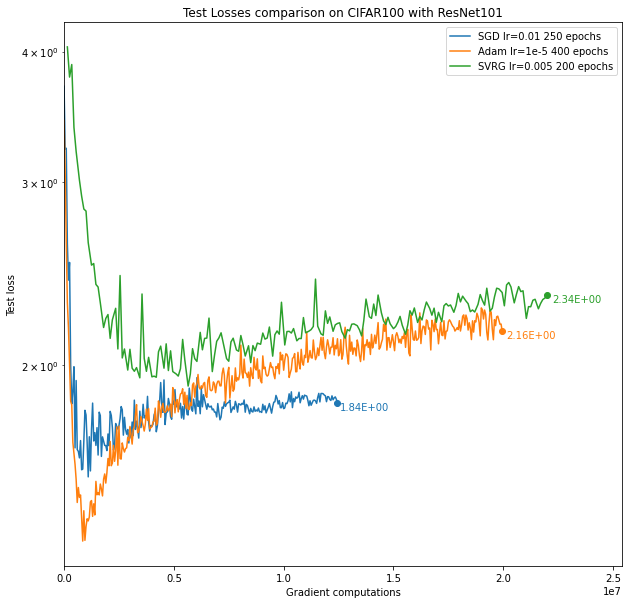
\includegraphics[scale=0.35]{report/figures/ResNet101Results.png}
         \label{fig:resnet101results}
     \end{figure}
\end{frame}

\begin{frame}{Results ResNet101 without BN}
      \begin{figure}
         \centering
         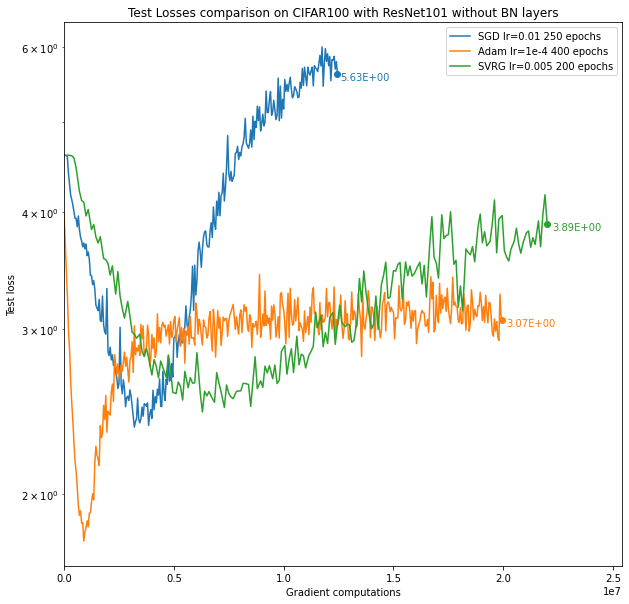
\includegraphics[scale=0.35]{report/figures/ResNet101noBNResults.png}
         \label{fig:resnet101noBNresults}
     \end{figure}
\end{frame}

\begin{frame}{MetaInit setup}
    \begin{itemize}
        \item We want to test whether using better weight initialization can help get better results in a setting without batch-normalization layers.
        \item Compare SVRG on ResNet101 without BN layers with and without MetaInit.
    \end{itemize}
    
    
\end{frame}

\begin{frame}{MetaInit results}
     \begin{figure}
         \centering
         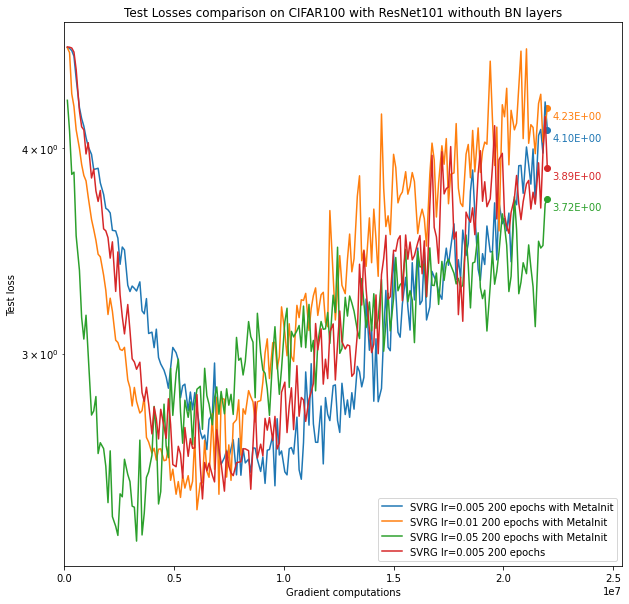
\includegraphics[scale=0.35]{report/figures/MetaInit_results_final.png}
         \label{fig:MetaInitresults}
     \end{figure}
\end{frame}

\begin{frame}{ }
    \begin{center}
        \Huge Conclusions
    \end{center}
\end{frame}

\begin{frame}{Conclusion}
    \begin{itemize}
        \pro Variance reduced methods are performing better than Adam and SGD on smaller architectures,
        \con VR methods outperformed on common deeper architectures with BN layers,
        \pro SVRG gets similar or better results than Adam and SGD when BN layers are removed,
        \con Searching for hyperparameters is harder without BN layers,
        \con Results without BN layers are not as good as with BN layers,
        \pro MetaInit helps for using bigger learning rates and get faster initial results.
        
    \end{itemize}
In summary, we seem to observe that SVRG is not disadvantaged as much as the other algorithms when removing batch-normalization layers from common DNNs but there are other unexplained phenomena that make the results somehow worse for all optimization algorithms.
\end{frame}

\begin{frame}{Available tools}
    \begin{itemize}
        \item Code for SVRG and STORM implementation and code for all experiments available in the repo of this project.
        \item Google Colab Notebook available to recreate experiments:
    \end{itemize}
    \begin{figure}
        \centering
        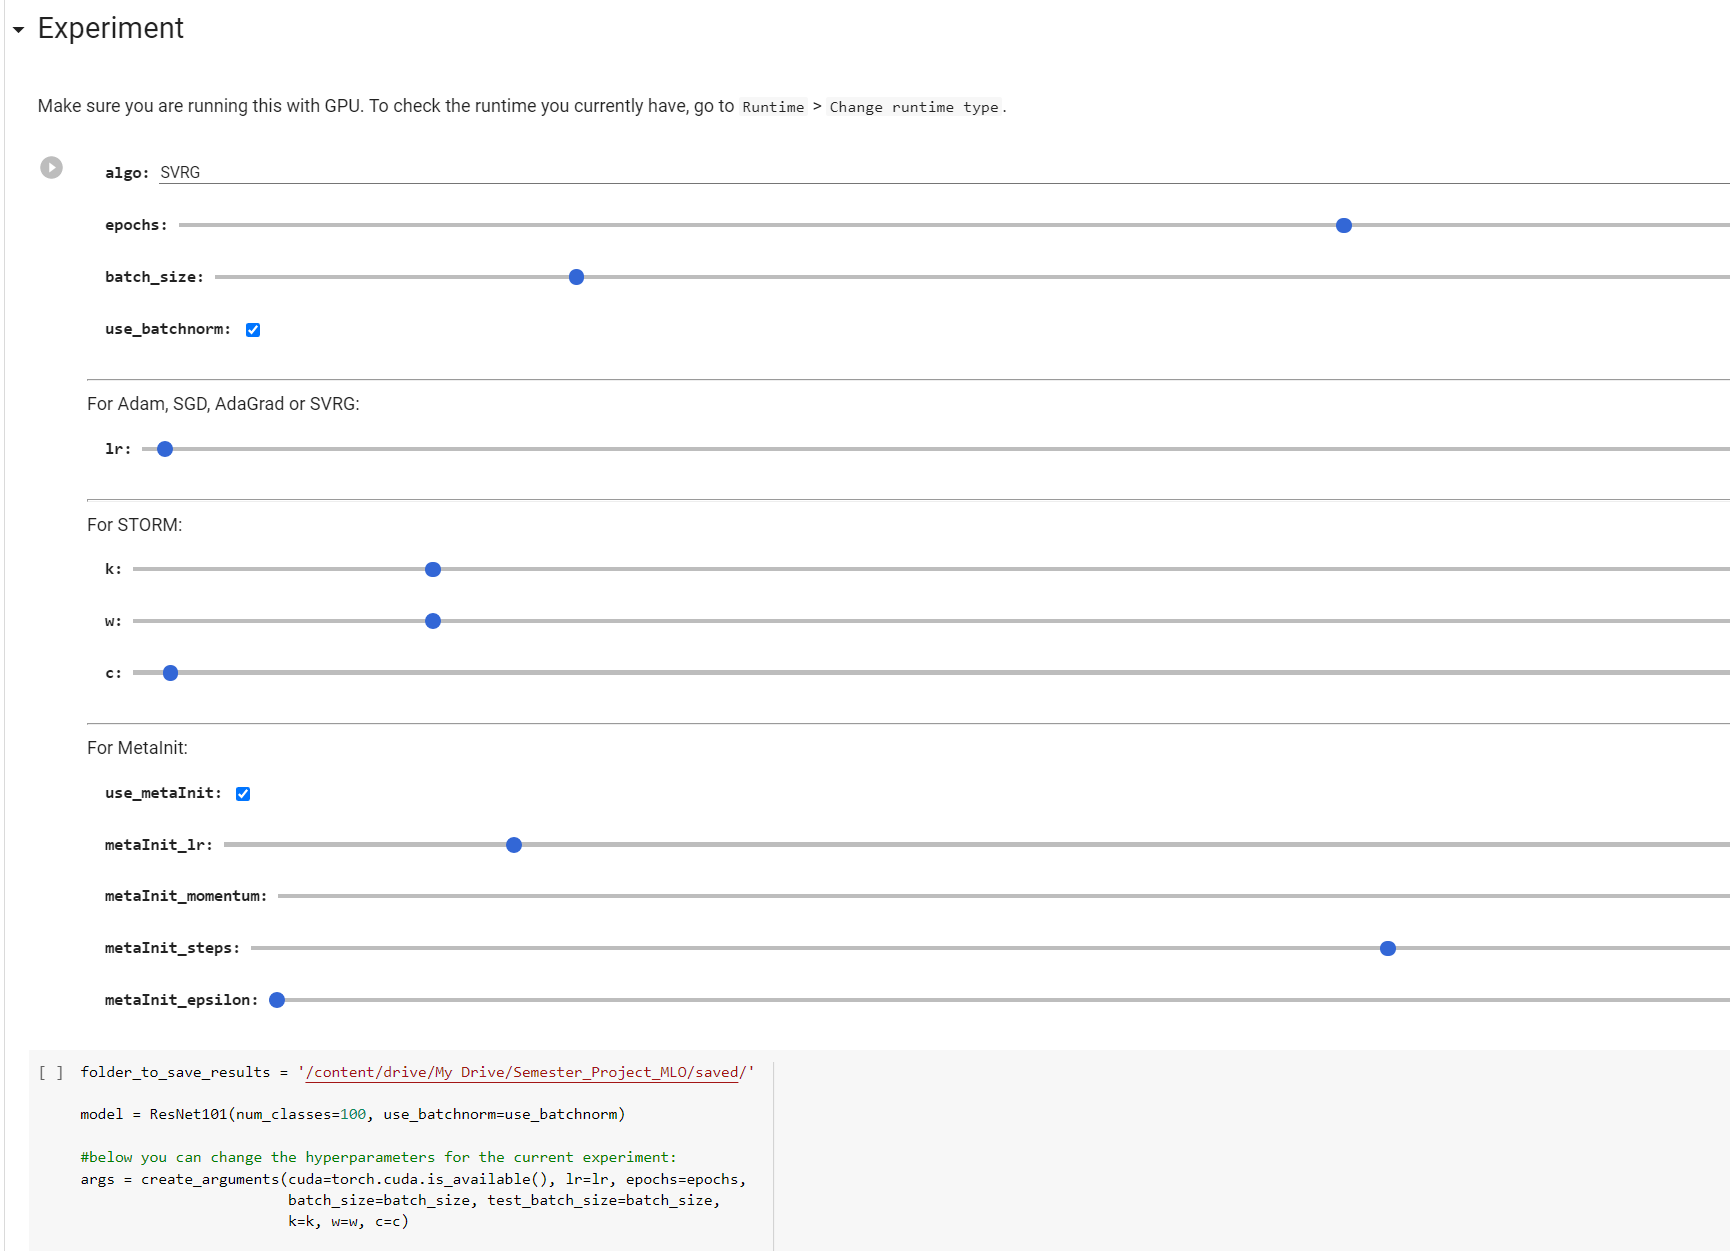
\includegraphics[width=.9\textwidth]{report/figures/ExampleExperiment.png}
    \end{figure}
\end{frame}

\begin{frame}{Future work}
    \begin{itemize}
        \item Proper Cross-validation for DNNs (with MetaInit),
        \item Test different DNNs, datasets and random seeds for more conclusive results.
    \end{itemize}
    
\end{frame}


\begin{frame}{ }
    \begin{center}
        \Huge Thank you\\ Any questions?
    \end{center}
\end{frame}


\begin{frame}[allowframebreaks]{References}
		\renewcommand*{\bibfont}{\tiny}
		\bibliography{presentation.bib}
   	% 	\bibliography{\jobname}
\end{frame}


%%%%%%%%%%%%%%%%%%%%%%%%%%%%%%%%%%%%%%%%%
%%%%%%%%%%%%%%% MORE SLIDES %%%%%%%%%%%%%
%%%%%%%%%%%%%%%%%%%%%%%%%%%%%%%%%%%%%%%%%

\begin{frame}{Additional Slides}
    \begin{center}
        \Huge Additional slides
    \end{center}
\end{frame}

\begin{frame}{Setup shallow NN}
    \begin{figure}
        \centering
    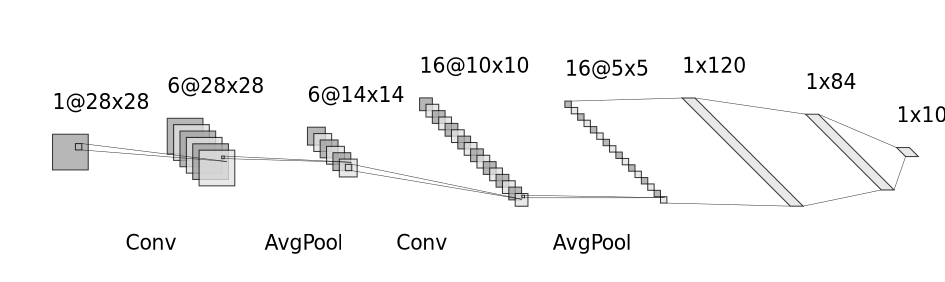
\includegraphics[scale=0.4]{report/midterm presentation/images/LeNet.png}
        \label{fig:lenet}
        \caption{LeNet network used for classification of MNIST}
    \end{figure} 
    \begin{figure}
        \centering
        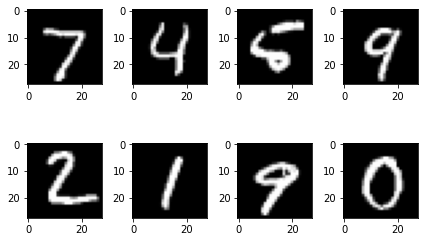
\includegraphics[width=.5\textwidth]{report/figures/MNIST_example.png}
        \caption{Example images of MNIST}
        \label{fig:MNIST_example}
    \end{figure}
\end{frame}

\begin{frame}{ResNet}
    Network for image recognition introduced in 2015~\citep{he2015residual}.
    
    \begin{figure}
        \centering
        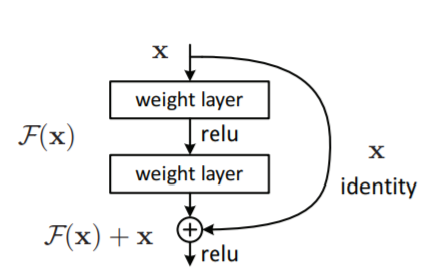
\includegraphics[scale=1]{report/midterm presentation/images/building_block_ResNet.png}
        \caption{Residual learning: a building block.}
        \label{fig:building_block_resnet}
    \end{figure}
    
    
\end{frame}

\begin{frame}{ResNet18}
    \begin{figure}
        \centering
        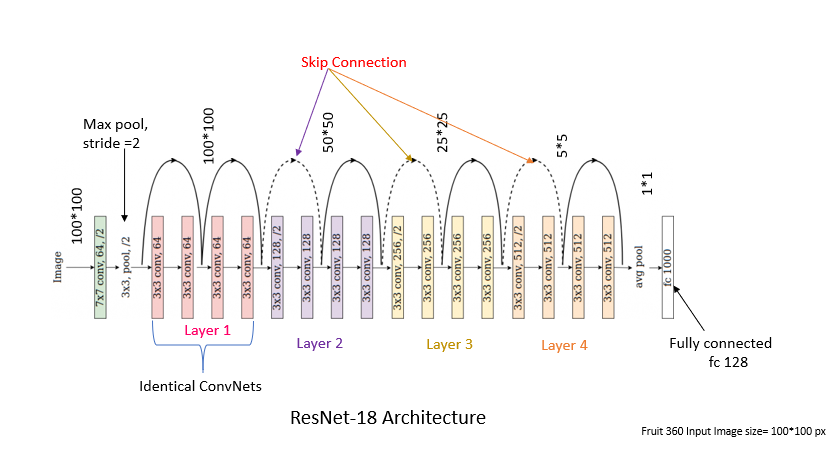
\includegraphics[scale=0.35]{report/midterm presentation/images/ResNet18.png}
        \label{fig:resnet18}
    \end{figure}
\end{frame}

\begin{frame}{Results on LeNet extended}
    \begin{figure}
        \centering
        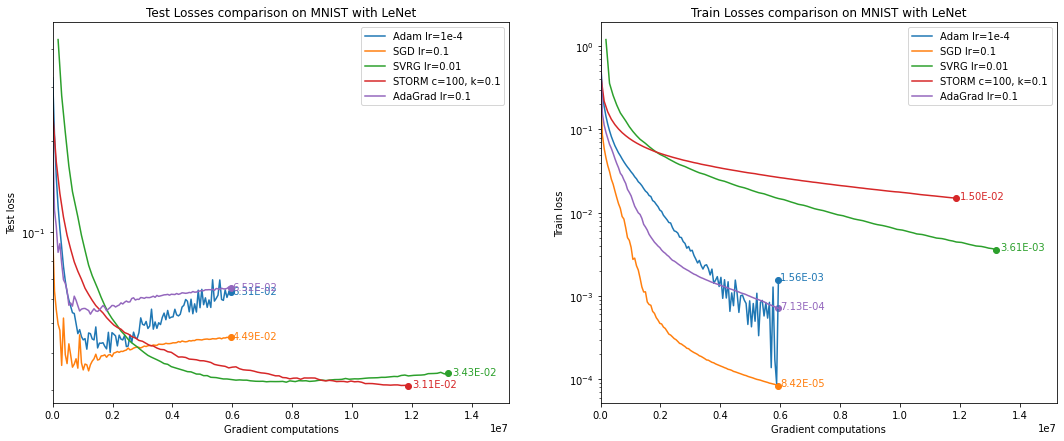
\includegraphics[width=\textwidth]{report/figures/MNIST.png}
        \caption{Test and train losses on LeNet for MNIST}
    \end{figure}
\end{frame}

\begin{frame}{Results on LeNet accuracies}
    \begin{table}[h]
    \begin{center}
        \begin{tabular}{||c | c | c||}
             \hline
             Algorithm & Test accuracy &  Train accuracy \\ \hline\hline
Adam & $0.9884$ & $0.9999$ \\ \hline
SGD & $0.9902$ & $1.0$ \\ \hline
SVRG & $0.9891$ & $0.9996$ \\ \hline
STORM & $0.9898$ & $0.9964$ \\ \hline
AdaGrad & $0.9859$ & $0.9999$ \\ \hline
        \end{tabular}
    \end{center}
    \end{table}
\end{frame}

\begin{frame}{Results ResNet18 extended}
    \begin{figure}
        \centering
        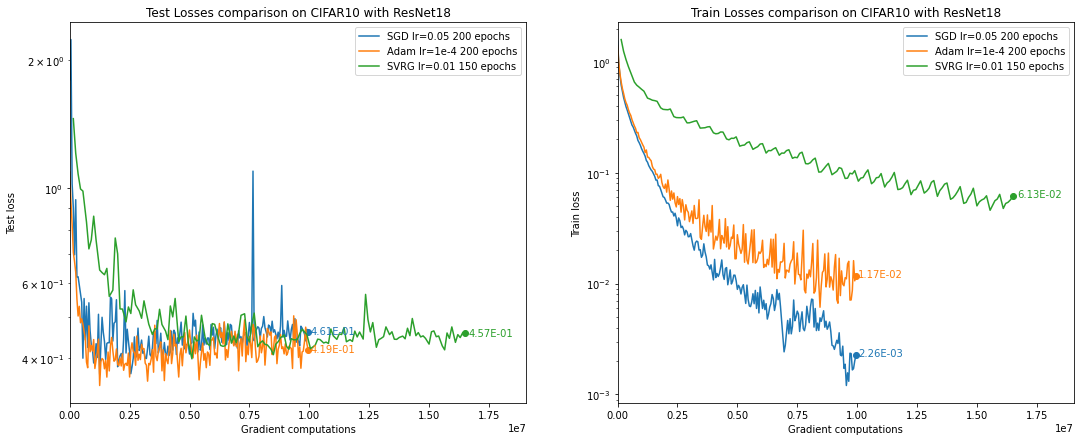
\includegraphics[width=\textwidth]{report/figures/CIFAR10.png}
    \end{figure}
\end{frame}

\begin{frame}{Results on ResNet18 accuracies}
    \begin{table}[h]
    \begin{center}
        \begin{tabular}{||c | c | c||}
             \hline
             Algorithm & Test accuracy &  Train accuracy \\ \hline\hline
SGD & $0.9221$ & $0.9996$ \\ \hline
ADAM & $0.9184$ & $0.9976$ \\ \hline
SVRG & $0.886$ & $0.97664$ \\ \hline

        \end{tabular}
    \end{center}
    \end{table}
\end{frame}

\begin{frame}{Results ResNet18 without BN layers extended}
    \begin{figure}
        \centering
        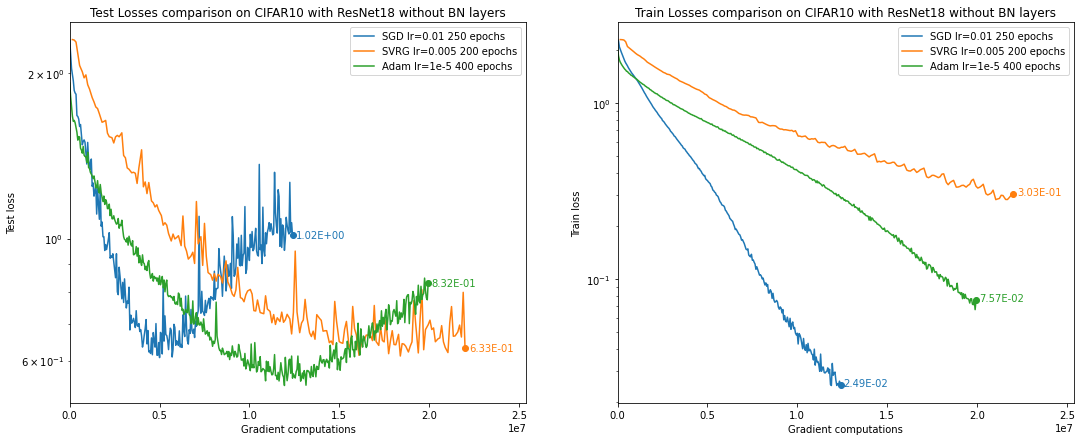
\includegraphics[width=\textwidth]{report/figures/CIFAR10noBN.png}
    \end{figure}
\end{frame}

\begin{frame}{Results on ResNet18 without BN layers accuracies}
    \begin{table}[h]
    \begin{center}
        \begin{tabular}{||c | c | c||}
             \hline
             Algorithm & Test accuracy &  Train accuracy \\ \hline\hline
SGD & $0.8382$ & $0.9924$ \\ \hline
ADAM & $0.8268$ & $0.9712$ \\ \hline
SVRG & $0.8044$ & $0.8990$ \\ \hline

        \end{tabular}
    \end{center}
    \end{table}
\end{frame}

\begin{frame}{Results ResNet101 extended}
    \begin{figure}
        \centering
        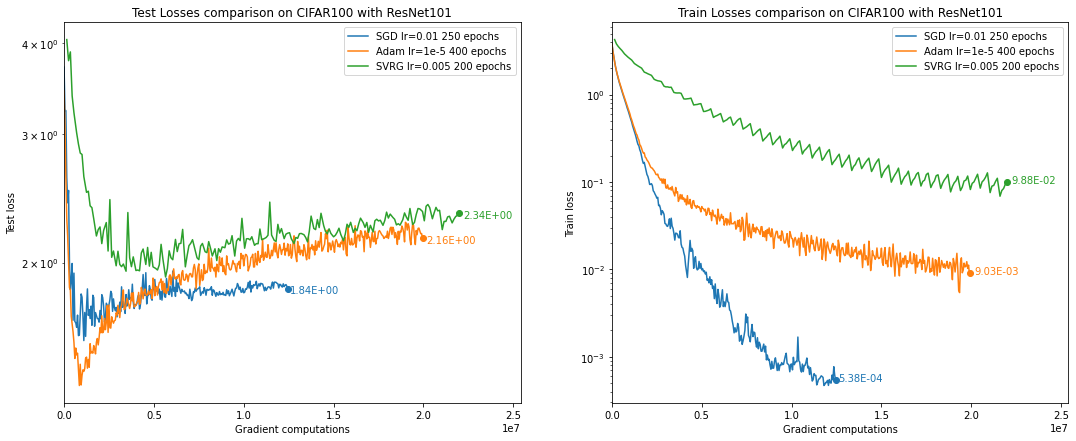
\includegraphics[width=\textwidth]{report/figures/CIFAR100.png}
    \end{figure}
\end{frame}

\begin{frame}{Results on ResNet101 accuracies}
    \begin{table}[h]
    \begin{center}
        \begin{tabular}{||c | c | c||}
             \hline
             Algorithm & Test accuracy &  Train accuracy \\ \hline\hline
SGD & $0.7239$ & $0.9999$ \\ \hline
ADAM & $0.7073$ & $0.9984$ \\ \hline
SVRG & $0.5947$ & $0.9734$ \\ \hline

        \end{tabular}
    \end{center}
    \end{table}
\end{frame}

\begin{frame}{Results ResNet101 without BN layers extended}
    \begin{figure}
        \centering
        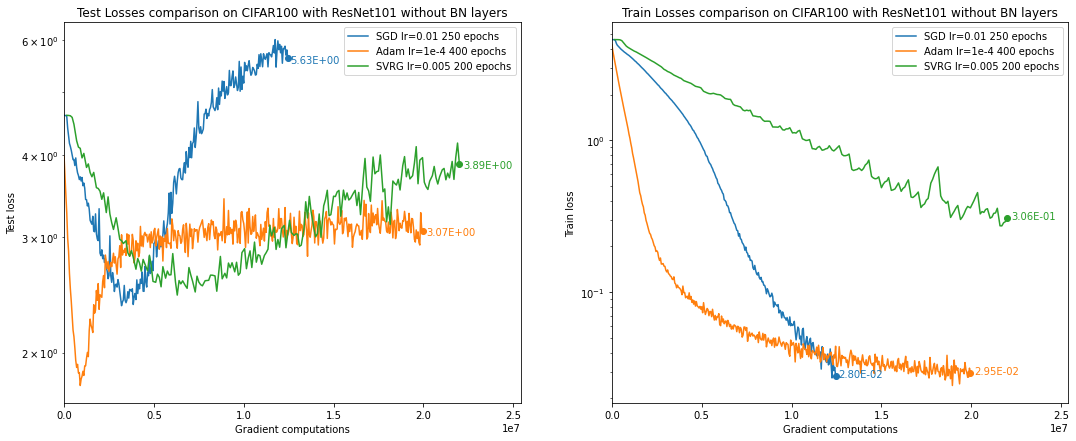
\includegraphics[width=\textwidth]{report/figures/CIFAR100noBN.png}
    \end{figure}
\end{frame}

\begin{frame}{Results on ResNet101 without BN layers accuracies}
    \begin{table}[h]
    \begin{center}
        \begin{tabular}{||c | c | c||}
             \hline
             Algorithm & Test accuracy &  Train accuracy \\ \hline\hline
SGD & $0.4771$ & $0.9925$ \\ \hline
ADAM & $0.6055$ & $0.9934$ \\ \hline
SVRG & $0.4441$ & $0.8915$ \\ \hline

        \end{tabular}
    \end{center}
    \end{table}
\end{frame}



\end{document}

